\documentclass[preprint,12pt,aps,pra,showkeys,amsmath,amssymb,superscriptaddress,floatfix]{revtex4-2}
\usepackage[T1]{fontenc}
\usepackage[utf8]{inputenc}
\usepackage{amsmath,amssymb,amsthm,mathtools,mathrsfs}
\usepackage{microtype,booktabs,enumitem}
\usepackage{xcolor,tikz,etoolbox}
\usepackage[skins,breakable]{tcolorbox}
\usepackage{needspace}
% Keep diagram geometry independent of REVTeX preprint body spacing.
\AtBeginEnvironment{tikzpicture}{\linespread{1}\selectfont}
\usetikzlibrary{arrows.meta,positioning,calc,fit,decorations.pathreplacing}
\usepackage{graphicx}
\usepackage{hyperref}

\definecolor{MMBlue}{RGB}{0,82,155}
\definecolor{MMOrange}{RGB}{200,80,0}
\tikzset{
 mmnode/.style={draw=MMBlue,rounded corners=2pt,fill=MMBlue!4,align=left,execute at begin node={\raggedright},text width=5cm,font=\fontsize{10}{12}\selectfont,inner sep=6pt},
 mmimport/.style={mmnode,draw=black!65,fill=black!4},
 mmcandidate/.style={mmnode,draw=MMOrange,dashed,fill=MMOrange!5},
 mmrejected/.style={mmnode,draw=black,densely dotted,fill=black!8},
 mmproof/.style={->,thick,MMBlue},
 mmflow/.style={->,semithick,black!70},
 mmrepair/.style={->,dashed,thick,MMOrange},
 mmcandidatearrow/.style={->,dashed,semithick,MMOrange},
 mmnote/.style={font=\scriptsize,fill=white,inner sep=2pt,align=center}}

\usepackage[section]{placeins}
\setlength{\emergencystretch}{3em}
\setlist{itemsep=3pt,topsep=4pt}
\newtheorem{theorem}{Theorem}[section]
\newtheorem{proposition}[theorem]{Proposition}
\newtheorem{lemma}[theorem]{Lemma}
\newtheorem{corollary}[theorem]{Corollary}
\theoremstyle{definition}
\newtheorem{definition}[theorem]{Definition}
\newtheorem{example}[theorem]{Example}
\theoremstyle{remark}
\newtheorem{remark}[theorem]{Remark}
% Avoid isolated statement headings and single-line paragraph fragments.
\BeforeBeginEnvironment{theorem}{\Needspace{6\baselineskip}}
\BeforeBeginEnvironment{definition}{\Needspace{5\baselineskip}}
\BeforeBeginEnvironment{proposition}{\Needspace{5\baselineskip}}
\BeforeBeginEnvironment{lemma}{\Needspace{5\baselineskip}}
\BeforeBeginEnvironment{corollary}{\Needspace{5\baselineskip}}
\clubpenalty=5000
\widowpenalty=5000
\newcommand{\R}{\mathbb R}\newcommand{\Z}{\mathbb Z}\newcommand{\N}{\mathbb N}
\newcommand{\Pa}{\operatorname{Pa}}\newcommand{\Desc}{\operatorname{Desc}}
\newcommand{\cl}{\operatorname{cl}}\newcommand{\cost}{\operatorname{cost}}
\newcommand{\status}{\operatorname{status}}
% Faculty cards: a visual rail groups the five faculties within one agent.
% The rail has no arrowhead and does not represent a proof dependency.
\newcommand{\mmfacultybadge}[1]{%
 \node[circle,draw=MMBlue,line width=1pt,fill=white,
 minimum size=7mm,inner sep=0pt,font=\sffamily\small\bfseries,text=MMBlue]
 at ([xshift=15pt,yshift=-15pt]frame.north west) {#1};}
\newcommand{\mmfacultyrail}{%
 \draw[MMBlue!80,line width=1pt]
 ([xshift=15pt,yshift=2pt]frame.north west)--
 ([xshift=15pt,yshift=-2pt]frame.south west);}
\newtcolorbox{mmfacultybox}[2]{enhanced,breakable,
 colback=MMBlue!4,colframe=MMBlue!4,boxrule=0pt,arc=3pt,
 left=39pt,right=9pt,top=4pt,bottom=4pt,
 before skip=2pt,after skip=2pt,
 fontupper=\small\linespread{1.1}\selectfont,
 overlay unbroken={\mmfacultyrail\mmfacultybadge{#1}},
 overlay first={\mmfacultyrail\mmfacultybadge{#1}},
 overlay middle={\mmfacultyrail},overlay last={\mmfacultyrail}}
\newcommand{\mmfaculty}[3]{%
 \begin{mmfacultybox}{#1}{#2}
 {\sffamily\bfseries\color{MMBlue}#2}\par\smallskip #3
 \end{mmfacultybox}}
\newcommand{\agent}[9]{%
 \Needspace{8\baselineskip}
 \subsubsection{#1}
 \noindent\textbf{Object.} #2\par
 \noindent\textbf{Role.} #3\par\smallskip
 \mmfaculty{E}{Ego}{#4}
 \mmfaculty{M}{Memory}{#5}
 \mmfaculty{I}{Intellect}{#6}
 \mmfaculty{S}{Sense}{#7}
 \mmfaculty{A}{Action}{#8}
 \smallskip\noindent #9\par}

\usepackage{longtable,array,calc}
\providecommand{\tightlist}{\setlength{\itemsep}{2pt}\setlength{\parskip}{0pt}}
\makeatletter
\def\frontmatter@abstract@produce{\par\addvspace{\frontmatter@preabstractspace}%
\begingroup\prep@absbox\unvbox\absbox\post@absbox\endgroup
\addvspace{\frontmatter@postabstractspace}}
\makeatother
\newcommand{\field}[2]{\par\smallskip\noindent\textbf{#1.} #2\par}
\setlength{\emergencystretch}{5em}
\AtBeginEnvironment{verbatim}{\small\linespread{1.0}\selectfont}


\hypersetup{colorlinks=true,linkcolor=MMBlue,urlcolor=MMBlue,pdfauthor={Dibakar Sigdel}}

\begin{document}

\title{Baire Category Theorem for Complete Metric Spaces\\[4pt]\large An End-to-End Meta-Math Walkthrough}

\author{Dibakar Sigdel}

\affiliation{Mindverse Computing LLC, Lynnwood, WA 98087, USA}

\date{October 2026}

\begin{abstract}

A complete authored walkthrough of baire category theorem for complete
metric spaces, with explicit mathematical contracts, local verification
gates, and reusable exports. The report presents the target theorem,
declared imports, a dependency graph, five-faculty node contracts, a
continuous proof, a worked example, and a hypothesis-repair audit. It is
an authored mathematical exposition, not a deployed-agent transcript or
a formal proof-assistant certificate.

\end{abstract}\maketitle\linespread{1.12}\selectfont

\noindent\textbf{GT-04 / General Topology / Report v1}

\section{Target and import contract}

\begin{theorem}

For a nonempty complete metric space \(X\), prove every countable
intersection of open dense subsets is dense. Equivalently, no nonempty
open subset is a countable union of nowhere dense subsets.

\end{theorem}

\subsection{Foundations and permitted imports}

X is a nonempty complete metric space. Dense means every nonempty open
set meets the set. Nowhere dense means the closure has empty interior.
Use the fact that every open neighborhood of a point contains a closed
ball of sufficiently small positive radius. Compactness of such balls is
not assumed.

\clearpage\section{Node interaction workflow}

\begin{center}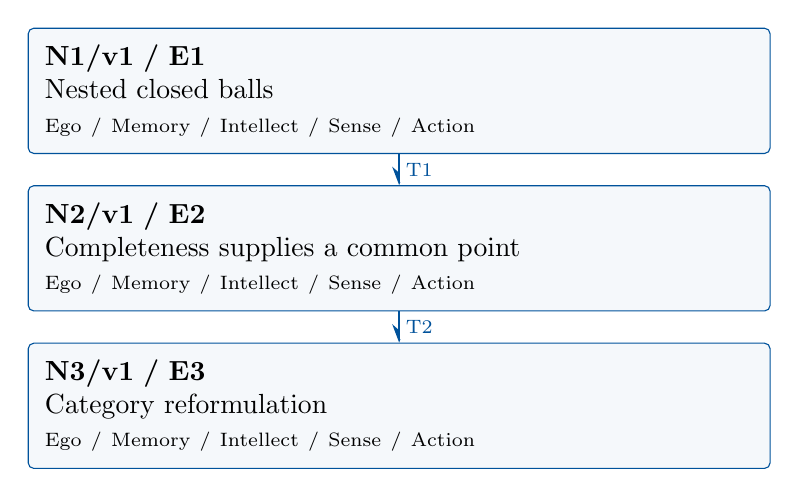
\begin{tikzpicture}[>=Stealth,x=1cm,y=1cm]

\node[mmnode,text width=9cm,minimum height=1.25cm] (N1) at (0,0.0) {\textbf{N1/v1 / E1}\\Nested closed balls\\{\scriptsize Ego / Memory / Intellect / Sense / Action}};

\node[mmnode,text width=9cm,minimum height=1.25cm] (N2) at (0,-2.0) {\textbf{N2/v1 / E2}\\Completeness supplies a common point\\{\scriptsize Ego / Memory / Intellect / Sense / Action}};

\node[mmnode,text width=9cm,minimum height=1.25cm] (N3) at (0,-4.0) {\textbf{N3/v1 / E3}\\Category reformulation\\{\scriptsize Ego / Memory / Intellect / Sense / Action}};

\draw[mmproof] (N1.south) -- node[mmnote,right] {T1} (N2.north);

\draw[mmproof] (N2.south) -- node[mmnote,right] {T2} (N3.north);

\end{tikzpicture}\end{center}

Each box is one mathematical agent containing all five faculties. Blue
arrows carry the versioned exports listed below. The layout gives a
reading order; only drawn arrows assert dependencies. Diagnostic repair
is separate from the proof DAG.

\subsection{Versioned evidence-transfer ledger}

\begingroup\small\linespread{1.05}\selectfont

\Needspace{5\baselineskip}\field{T1: N1/E1/v1 to N2}{Nested nonempty closed balls with radii tending to 0 and all required
inclusions.}

\field{Receiving activity}{N2: Completeness supplies a common point}

\field{Compatibility}{Use the same mathematical objects and hypotheses as the source export.
Receiving contract: Nested balls and shrinking radii; prior exports
E1/v1}

\Needspace{5\baselineskip}\field{T2: N2/E2/v1 to N3}{Every countable intersection of open dense sets is dense.}

\field{Receiving activity}{N3: Category reformulation}

\field{Compatibility}{Use the same mathematical objects and hypotheses as the source export.
Receiving contract: Dense-intersection theorem and nowhere-dense
definition; prior exports E2/v1}

\endgroup

\clearpage\section{Agent roles and five-faculty activities}\begingroup\small\linespread{1.05}\selectfont\setlist{itemsep=1pt,topsep=2pt}

\subsection{N1/v1: Nested closed balls}

\field{Object and role}{Place each next ball inside the previous interior and the next dense
open set.}

\field{Inputs}{Open dense \(G_{1},G_{2},\ldots\); arbitrary nonempty open U;
foundational imports stated in §1}

\mmfaculty{E}{Ego}{Own E1/v1: Nested nonempty closed balls with radii tending to 0 and all
required inclusions.}

\mmfaculty{M}{Memory}{Retain Open dense \(G_{1},G_{2},\ldots\); arbitrary nonempty open U;
foundational imports stated in §1; keep their assumptions and versions
attached.}

\mmfaculty{I}{Intellect}{Place each next ball inside the previous interior and the next dense
open set.}

\mmfaculty{S}{Sense}{Do not invoke compactness of closed balls in a general complete metric
space.}

\mmfaculty{A}{Action}{Carry out the numbered deductions and publish E1/v1 together with its
hypotheses and proof location.}

\smallskip\noindent\textbf{Numbered mathematical activities}

\begin{enumerate}[label=N1.\arabic*,leftmargin=3.4em]

\item Choose a positive-radius closed ball \(B_{1}\) contained in
\(U\cap G_{1}\), with \(r_{1}\le 1/2\).

\item This intersection is nonempty open.

\item Inductively the open ball centered at \(x_n\) with radius \(r_n\) meets
\(G_{n+1}\); choose a point there and a positive radius
\(r_{n+1}\le 2^{(-n-1)}\) so its closed ball \(B_{n+1}\) is contained in
that intersection.

\item Then \(B_{n+1}\subset B_n\) and
\(B_n\subset U\cap G_{1}\cap \cdots \cap G_n\).

\item This works also at isolated points, where small balls may be singletons.

\end{enumerate}

\field{Export E1/v1}{Nested nonempty closed balls with radii tending to 0 and all required
inclusions.}

\field{Acceptance gate}{Do not invoke compactness of closed balls in a general complete metric
space. Publish only after checking every displayed deduction.}

\field{Targeted repair}{If the check fails, revise N1: Do not invoke compactness of closed balls
in a general complete metric space. Recheck dependent nodes N2, N3.}

\clearpage

\subsection{N2/v1: Completeness supplies a common point}

\field{Object and role}{Control centers by nesting and use closedness.}

\field{Inputs}{Nested balls and shrinking radii; prior exports E1/v1}

\mmfaculty{E}{Ego}{Own E2/v1: Every countable intersection of open dense sets is dense.}

\mmfaculty{M}{Memory}{Retain Nested balls and shrinking radii; prior exports E1/v1; keep their
assumptions and versions attached.}

\mmfaculty{I}{Intellect}{Control centers by nesting and use closedness.}

\mmfaculty{S}{Sense}{Vanishing consecutive increments alone would not have supplied this
Cauchy estimate.}

\mmfaculty{A}{Action}{Carry out the numbered deductions and publish E2/v1 together with its
hypotheses and proof location.}

\smallskip\noindent\textbf{Numbered mathematical activities}

\begin{enumerate}[label=N2.\arabic*,leftmargin=3.4em]

\item For \(m>n\), \(x_m\) lies in \(B_n\), so \(d(x_m,x_n)\le r_n\to 0\).

\item Thus the centers are Cauchy and converge to \(x\in X\) by completeness.

\item For fixedn, all subsequent centers lie in the closed set \(B_n\), so
\(x\in B_n\).

\item Consequentlyx lies in U and every \(G_n\).

\item Since U was any nonempty open set, \(\cap G_n\) is dense.

\end{enumerate}

\field{Export E2/v1}{Every countable intersection of open dense sets is dense.}

\field{Acceptance gate}{Vanishing consecutive increments alone would not have supplied this
Cauchy estimate. Publish only after checking every displayed deduction.}

\field{Targeted repair}{If the check fails, revise N2: Vanishing consecutive increments alone
would not have supplied this Cauchy estimate. Recheck dependent nodes
N3.}

\clearpage

\subsection{N3/v1: Category reformulation}

\field{Object and role}{Take complements of closures.}

\field{Inputs}{Dense-intersection theorem and nowhere-dense definition; prior exports
E2/v1}

\mmfaculty{E}{Ego}{Own E3/v1: The stated Baire theorem and category equivalence.}

\mmfaculty{M}{Memory}{Retain Dense-intersection theorem and nowhere-dense definition; prior
exports E2/v1; keep their assumptions and versions attached.}

\mmfaculty{I}{Intellect}{Take complements of closures.}

\mmfaculty{S}{Sense}{The relevant sets are nowhere dense, not merely empty-interior sets
without a closure check.}

\mmfaculty{A}{Action}{Carry out the numbered deductions and publish E3/v1 together with its
hypotheses and proof location.}

\smallskip\noindent\textbf{Numbered mathematical activities}

\begin{enumerate}[label=N3.\arabic*,leftmargin=3.4em]

\item If \(A_n\) are nowhere dense, \(G_n=X\setminus\operatorname{cl}(A_n)\)
are open dense.

\item Their intersection meets every nonempty open U, so U cannot be covered
by \(\cup A_n\).

\item Conversely, if some open dense \(G_n\) have intersection missing a
nonempty open U, then \(U\subset \cup (X\setminus G_n)\), each
complement closed with empty interior, contradicting the category
property.

\item Thus the formulations are equivalent.

\end{enumerate}

\field{Export E3/v1}{The stated Baire theorem and category equivalence.}

\field{Acceptance gate}{The relevant sets are nowhere dense, not merely empty-interior sets
without a closure check. Publish only after checking every displayed
deduction.}

\field{Targeted repair}{If the check fails, revise N3: The relevant sets are nowhere dense, not
merely empty-interior sets without a closure check. Withhold this
terminal result until its gate passes.}

\endgroup\clearpage\section{Continuous mathematical proof}\label{sec:proof}

Read these steps in order as one proof; the diagram is optional.
Numbered activities identify the specific constructions and deductions
owned by each node.

\subsection{§4.N1 --- Nested closed balls}\label{n1-nested-closed-balls}

Fix a nonempty open set \(U\) and a sequence of open dense sets \(G_n\).

\begin{enumerate}
\def\labelenumi{\arabic{enumi}.}
\item
  Choose a positive-radius closed ball \(B_{1}\) contained in
  \(U\cap G_{1}\), with \(r_{1}\le 1/2\).
\item
  This intersection is nonempty open.
\item
  Inductively the open ball centered at \(x_n\) with radius \(r_n\)
  meets \(G_{n+1}\); choose a point there and a positive radius
  \(r_{n+1}\le 2^{(-n-1)}\) so its closed ball \(B_{n+1}\) is contained
  in that intersection.
\item
  Then \(B_{n+1}\subset B_n\) and
  \(B_n\subset U\cap G_{1}\cap \cdots \cap G_n\).
\item
  This works also at isolated points, where small balls may be
  singletons.
\end{enumerate}

\subsection{§4.N2 --- Completeness supplies a common
point}\label{n2-completeness-supplies-a-common-point}

\begin{enumerate}
\def\labelenumi{\arabic{enumi}.}
\item
  For \(m>n\), \(x_m\) lies in \(B_n\), so \(d(x_m,x_n)\le r_n\to 0\).
\item
  Thus the centers are Cauchy and converge to \(x\in X\) by
  completeness.
\item
  For fixedn, all subsequent centers lie in the closed set \(B_n\), so
  \(x\in B_n\).
\item
  Consequentlyx lies in U and every \(G_n\).
\item
  Since U was any nonempty open set, \(\cap G_n\) is dense.
\end{enumerate}

\subsection{§4.N3 --- Category
reformulation}\label{n3-category-reformulation}

\begin{enumerate}
\def\labelenumi{\arabic{enumi}.}
\item
  If \(A_n\) are nowhere dense, \(G_n=X\setminus\operatorname{cl}(A_n)\)
  are open dense.
\item
  Their intersection meets every nonempty open U, so U cannot be covered
  by \(\cup A_n\).
\item
  Conversely, if some open dense \(G_n\) have intersection missing a
  nonempty open U, then \(U\subset \cup (X\setminus G_n)\), each
  complement closed with empty interior, contradicting the category
  property.
\item
  Thus the formulations are equivalent.
\end{enumerate}

\hfill$\square$

\section{Worked orchestration}

In R, enumerate rationals \(q_n\) and set \(G_n=R\setminus\{q_n\}\).
Their intersection is the irrationals, which the theorem shows are
dense. Each \(G_n\) is open dense; the argument constructs an irrational
inside any chosen nonempty interval.

\subsection{Boundary and hypothesis audit}

Q with its usual metric is incomplete and is the countable union of
singleton nowhere-dense subsets relative to Q. The complements of its
enumerated points have empty total intersection. Sense traces the
failure to the missing metric limit in X, not to the finite nesting
steps.

\section{Illustrative failure and repair}

The following is an authored diagnostic scenario. Changed assumptions
define a new contract; they do not retroactively prove the original
statement.

\subsection{Failure and correction}
This is an authored teaching trace, not a recorded agent run.

\begin{enumerate}
\def\labelenumi{\arabic{enumi}.}
\tightlist
\item
  \textbf{Ego \(\to\) Memory:} register the §1 theorem, imports, and
  requested exports before beginning the proof.
\item
  \textbf{Intellect \(\to\) Action:} choose the bridges in §3 and carry
  out the numbered activities in §4; transmit only established E-exports
  along the §2 DAG.
\item
  \textbf{Sense \(\to\) responsible node:} test the specific
  boundary/failure in §5 and the node's individual audit. A failing
  candidate is withheld; downstream nodes may not use it.
\item
  \textbf{Memory + Intellect:} identify whether the error is an omitted
  condition, an invalid inference, or an attempted extension beyond the
  theorem. Restore the exact contract or explicitly state a different
  one.
\item
  \textbf{Action:} redo the affected mathematical activity using the
  repaired condition or inference. Recheck consuming nodes, rather than
  feeding their conclusions back as premises.
\item
  \textbf{Ego:} publish only the supported export with its assumptions
  and proof location. A hypothetical revised export is v2; the written
  proof here is the v1 exposition, not a claim that this repair was
  executed.
\end{enumerate}

\subsection{Hypothesis boundary}
Q with its usual metric is incomplete and is the countable union of
singleton nowhere-dense subsets relative to Q. The complements of its
enumerated points have empty total intersection. Sense traces the
failure to the missing metric limit in X, not to the finite nesting
steps.

\subsection{Version and recheck}
Treat any changed assumption as a new contract. Recheck the revised
export and all of its descendants. A backward diagnostic never
establishes an earlier theorem. This is an authored teaching trace, not
an execution log.

\par\medskip\begingroup\small\linespread{1.0}\selectfont\noindent\textbf{Provenance.} This authored proof is complete relative to its declared imports. Reuse
each export with its assumptions, proof, and version. The original
Markdown remains available for comparison.
\par\endgroup

\par\smallskip\begingroup\small\linespread{1.0}\selectfont\noindent\textbf{Further reading.} \begin{itemize}
\tightlist
\item
  \href{https://ocw.mit.edu/courses/18-901-introduction-to-topology-fall-2004/pages/lecture-notes/}{MIT
  Introduction to Topology: separation, Urysohn, and Tychonoff
  material}.
\end{itemize}\par\endgroup

\end{document}
